\section{Introduction}
\label{sec:introduction}

In traditional robotics applications such as pick and place, spray-painting and spot-welding, the robots either do not need very high accuracy or they are programmed by teaching, where the \textbf{repeatability} of the robot is more important than the \textbf{accuracy}. Repeatability refers to the robot's capability to return precisely to the same location as previously taught, whereas accuracy refers to the robot's capability to precisely reach a pose computed based on the robot's kinematic model. 

However, there are many applications where the accuracy of the robot becomes very crucial, given that the robot has to adapt to each task automatically with a great precision. Consider, for example, a robot drilling task in \cite{Suarez-Ruiz2018} where the robot is supposed to drill several holes at precisely-defined locations on a workpiece. The workpiece can be different for each task, and the placement within the workspace may not be precisely known. Programming by teaching in this case requires manual re-programming for each workpiece which is very inefficient. To program the robot automatically for such task, the robot has to do a few things accurately: the robot has to scan the workpiece, determine the location of the holes, and finally move to that location accurately. The accuracy of such a robotic system depends on at least two things: The accuracy of the robot and the accuracy of the measurement system. 
\begin{figure}[t]
  \centering
  \vspace*{2mm}
  \subfloat[]{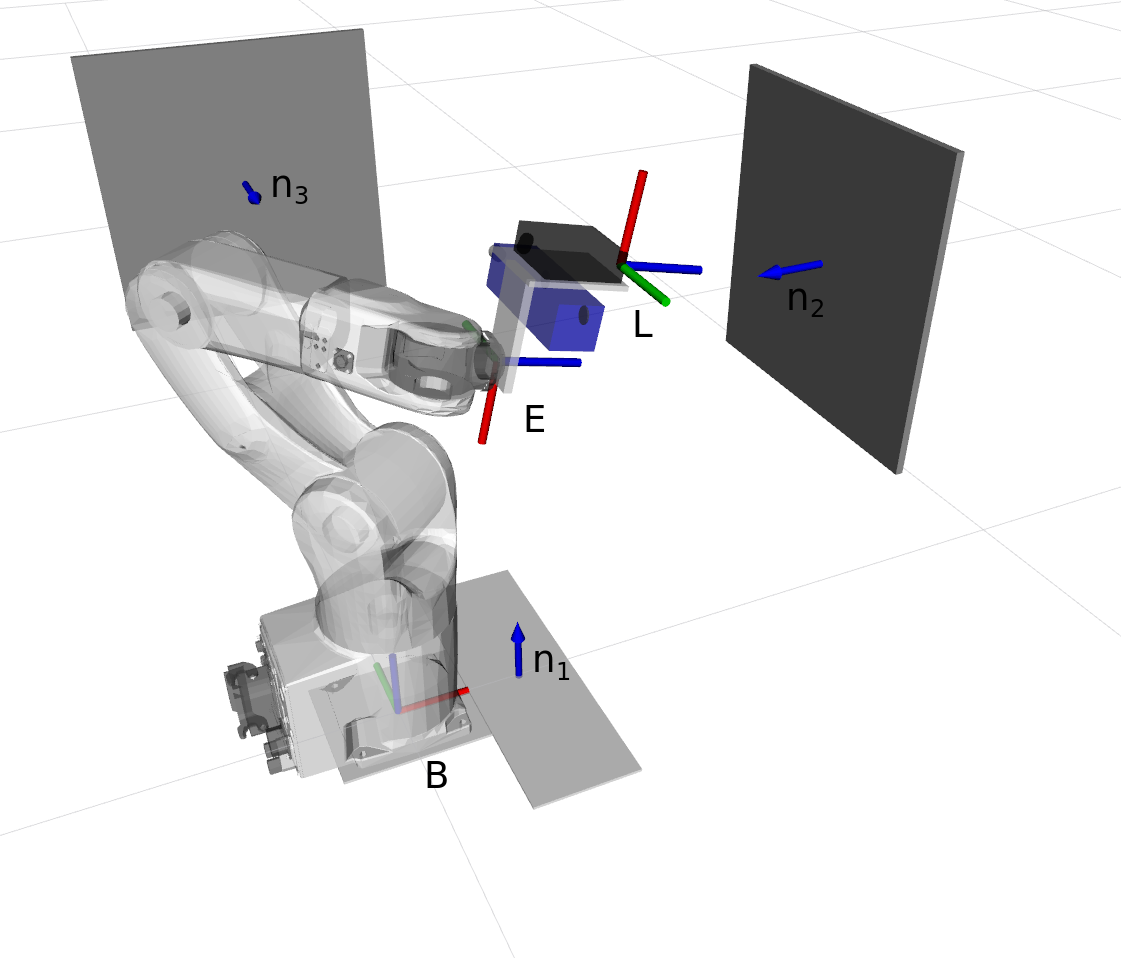
\includegraphics[height=60mm]{robot_setup}}
  \caption{Calibration Setup}
  \label{fig:robot_setup}
\end{figure}

The accuracy of the robot is determined by how closely the kinematic parameters of the robot's model resemble the actual kinematic parameters of the physical robot. This is affected by the manufacturing process, the assembly process, and the wear and tear during the operation of the robot. \textbf{Robot kinematic calibration} is usually conducted to achieve a better accuracy, either by using an external measurement system (such as motion capture system or coordinate measuring machines) or by constraining the motion of the end-effector.

The accuracy of the measurement system can be divided into two parts: the accuracy of the measurement device itself and the accuracy of the relative pose between the robot frame and the measurement frame. The accuracy of the measurement device depends on the type of device that is used and its specification. For example, a camera system is generallly less precise as compared to a laser system, although a camera can give more information. The second part of the accuracy comes from the fact that the data from a measurement system is always obtained in the measurement device coordinate frame, and it needs to be transformed to the robot coordinate system. Hence, the relative pose between the robot coordinate frame and the measurement device frame needs to be obtained. This relative pose is often called the \textbf{extrinsic parameters} of the measurement device, and the method to estimate the extrinsic parameters is called \textbf{extrinsic calibration}.  


\renewcommand{\arraystretch}{1.3}
\begin{table*}[htp]
\caption{Examples of Unconstrained Calibration}
\label{tab:unconstrained_calib}
\centering
\begin{tabular}{c c c c c}
\toprule
\textbf{Researchers} &  \textbf{Robot} & \textbf{Measurement Device} &  \textbf{Initial Accuracy[mm]}  & \textbf{Final Accuracy[mm]}\\
\midrule
Ginani and Mota \cite{Ginani2011} & ABB IRB 2000 & ROMER Measurement Arm & 2.20 & 1.40 \\
Ye et al. \cite{Ye2006} & ABB IRB 2400/L & Faro Laser Tracker & 1.764 & 0.640 \\
Nubiola and Bonev \cite{Nubiola2013} & ABB IRB 1600-6/1.45 & Faro Laser Tracker ION & 2.158 & 0.696 \\ 
Newman et al. \cite{Newman2000} & Motoman P-8 & SMX Laser Tracker & 3.595 & 2.524\\
\bottomrule
\end{tabular}
\end{table*}



In this paper we present SCALAR, a calibration method to simultaneously improve the accuracy of the robot and the measurement system. SCALAR calibrates simultaneously the kinematic parameters of the robot and the extrinsic parameters of a 2D \acl{lrf} (\ac{lrf}) using only the information provided by the \ac{lrf} attached to the robot end-effector. An \ac{lrf} is chosen because it gives very accurate measurement data both for the calibration and for the subsequent tasks (such as drilling).  

The overall calibration procedure is as follows:
\begin{enumerate}
\item The \ac{lrf} is attached to the robot and three perpendicular planes are placed around the robot as shown in \fref{fig:robot_setup}. Only the rough estimate of the position and orientation of the planes are necessary to be known, so the setup can be easily done.
\item For each plane, the robot is moved to several poses such that the \ac{lrf}'s 2D ray is projected onto the plane. The data from the \ac{lrf} as well as the robot's joint angles information are collected.
\item An optimization algorithm is used to find the optimal robot's kinematic parameters together with the \ac{lrf} extrinsic parameters, using the geometric constraint that the projected \ac{lrf} data should be located on the three planes. 
\end{enumerate}

The remainder of the paper is as follows. In \sref{sec:related} we discuss the existing approaches to the calibration problem both for the robot's kinematic parameters and the \ac{lrf}'s extrinsic parameters, and how SCALAR differs from the other approaches. In \sref{sec:method}, SCALAR is explained in detail. A simulation study is presented in \sref{sec:simulation} to verify SCALAR, and finally we conclude with a few remarks in \sref{sec:conclusions}.  



\section{Related works}
\label{sec:related}
\subsection{Calibration of robot's kinematic parameters}
\label{sec:kine_calib}



Robot kinematic calibration has been researched for a long time; some of the earliest works began in 1980s. The calibration procedures can be categorized into unconstrained and constrained calibration. In unconstrained calibration, the robot moves its end-effector to several poses while an external measurement system measures the pose. The measured pose is then compared to the one computed from the kinematic model, and the model is updated to minimize the difference between the predicted pose and the measured pose. In constrained calibration, some constraints are applied to the motion of the end-effector, and the constraints yield several calibration equations by which the robot's kinematic parameters are calibrated. 


Examples of unconstrained calibration works can be seen in \tref{tab:unconstrained_calib}. The issues with such calibration method are the difficulty in setting up the calibration setup and the expensive cost of the external measurement system. For example, the cost of a laser tracker is more than $\$100,000$ USD \cite{Nubiola2013}. Therefore, many researchers try to find calibration methods which only rely on the internal sensors of the robot by constraining the motion of the end-effector such as in constrained calibration. 

In \cite{Ikits1997}, Ikits and Hollerbach propose a kinematic calibration method using a planar constraint. A touch probe attached to the robot's flange is moved to touch random points on a plane. When the touch probe is in contact with the plane, the joint angles are recorded. The kinematic parameters of the robot model are then updated to satisfy the planar constraint. While the approach is promising, they also report that some of the parameters are hardly observable when the measurements are noisy or when the model is not complete. The unobservability of the parameters means that some of the parameters cannot be obtained accurately from the calibration procedure.

In \cite{Zhuang1999}, Zhuang et al. investigate robot calibration with planar constraints, in particular the observability conditions of the robot's kinematic parameters. They prove that a single-plane constraint is insufficient for calibrating a robot, and a minimum of three planar constraints are necessary. Using three planar constraints, the constrained system is proved to be equivalent to an unconstrained point-measurement system under three conditions: a) All three planes are mutually non-parallel, b) the identification Jacobian of the unconstrained system is nonsingular, and c) the measured points from each individual plane do not lie on a line on that plane. They verify the theory by doing a simulation on a PUMA560 robot. 

In \cite{Joubair2015}, Joubair and Bonev calibrated both the kinematic and non-kinematic (stiffness) parameters of a FANUC LR Mate 200iC industrial robot by using planar constraints, in the form of a high precision 9-inches granite cube. The robot is equipped with an MP250 Renishaw touch probe, which is then moved to touch four planes of the granite cube. The granite cube's face is flat to within 0.002mm. They improved the maximum plane error from 3.740mm to 0.083mm. 

\subsection{Calibration of extrinsic 2D \ac{lrf} parameters}
\label{sec:laser_calib}
Extrinsic calibration of an \ac{lrf} consists of finding the correct homogeneous transformation from the robot coordinate frame to the laser coordinate frame. Most of the works on extrinsic calibration of an \ac{lrf} involves a camera, since both sensors are often used together in many applications. The works in this field are largely based on Zhang and Pless' work \cite{Zhang2004}. They propose a method to calibrate both a camera and an \ac{lrf} using a planar checkerboard pattern. First, the camera is calibrated by a standard hand-eye calibration  \cite{BouguetJ.Y.2003} using a checkerboard pattern. The calibrated camera is then used to calculate the pose of the pattern. Next, the robot is moved to several poses with the \ac{lrf} pointing to the pattern. By using the geometric constraints that all the data points from the \ac{lrf} should fall on the pattern plane, the extrinsic parameters of the \ac{lrf} can be obtained. Finally, the same constraints are used to optimize both the intrinsic and extrinsic parameters of the camera and the extrinsic parameters of the \ac{lrf}. The nonlinear optimization problem is solved by using Levenberg-Marquardt optimization algorithm.

Unnikrishnan and Hebert \cite{Unnikrishnan2005} use the same setup as \cite{Zhang2004}, although they do not optimize the camera parameter simultaneously due to the nonlinearity of the resulting cost function. 
Li et al. \cite{Li2007} use a specially designed checkerboard to calibrate the extrinsic parameters between a camera and an \ac{lrf}, and claim that the result is better than \cite{Zhang2004}. Vasconcelos et al. \cite{Vasconcelos2012} develop a minimal closed-form solution for the extrinsic calibration of a camera and an \ac{lrf}, based on the work in \cite{Zhang2004}. 

\subsection{Novelty of the proposed method}
\label{sec:novelty}
SCALAR can be seen as a combination of the algorithm for extrinsic calibration of an \ac{lrf} \cite{Zhang2004} and the algorithm for calibration of robot's kinematic parameters using three planar constraints \cite{Joubair2015}. It has the following advantages as compared to the other calibration approaches:
\begin{enumerate}
\item SCALAR simultaneously calibrates both the \ac{lrf} extrinsic parameters and the robot's kinematic parameters. Given that calibration process is often cumbersome, this saves a lot of time and effort. Moreover, the errors in the robot's kinematic parameters affect the extrinsic calibration accuracy, and vice versa. Hence, calibrating both parameters simultaneously results in better accuracy. 
\item SCALAR does not need an additional camera to calibrate the \ac{lrf}, unlike \cite{Zhang2004}.
\item SCALAR does not need another expensive external measurement system. The measurement is done using the \ac{lrf} that will also be used in the subsequent robot task, hence it does not incur additional cost. Moveover, an \ac{lrf} can achieve very high accuracy at much lower cost (more than ten times cheaper) as compared to the commonly used measurement systems such as Vicon or Faro Laser Tracker. 
\item SCALAR does not need a precisely manufactured calibration object such as the granite cube in \cite{Joubair2015}, which requires the planes' position and orientation to be known accurately. SCALAR only requires
three flat surfaces which are oriented roughly perpendicular to each other and the rough estimate of their locations. This also means that the calibration setup can be done easily.
\item The calibration poses can be distributed throughout the whole workspace, instead of being confined only in a local region such as in \cite{Joubair2015}. 
\end{enumerate}



%%% Local Variables:
%%% mode: latex
%%% TeX-master: "../main"
%%% End:
